\subsection{Overview}
 Here the architectural elements that compose the system are explained with their interaction. A description of the replication mechanism chosen in order to make the system distributed is also given.
The architectural framework adopted by the CKB platform needs to be robust and scalable. A three-tier application model is used, since it guarantees several of the nonfunctional requirements previously described in the RASD, such as reliability, since having several components which perform the same activity renders the system fault-tolerant, and maintainability, because having a system divided into three layers, any of which independent from the other ones, ensures atomicity between their functionalities. In addition, each tier runs on its own infrastructure, so can be developed individually and simultaneously with the others, giving flexibility and scalability to the system.
This architectural paradigm consists of three tiers: the presentation tier, the application logic tier, and the data storage tier.

\begin{figure}[H]
    \centering
    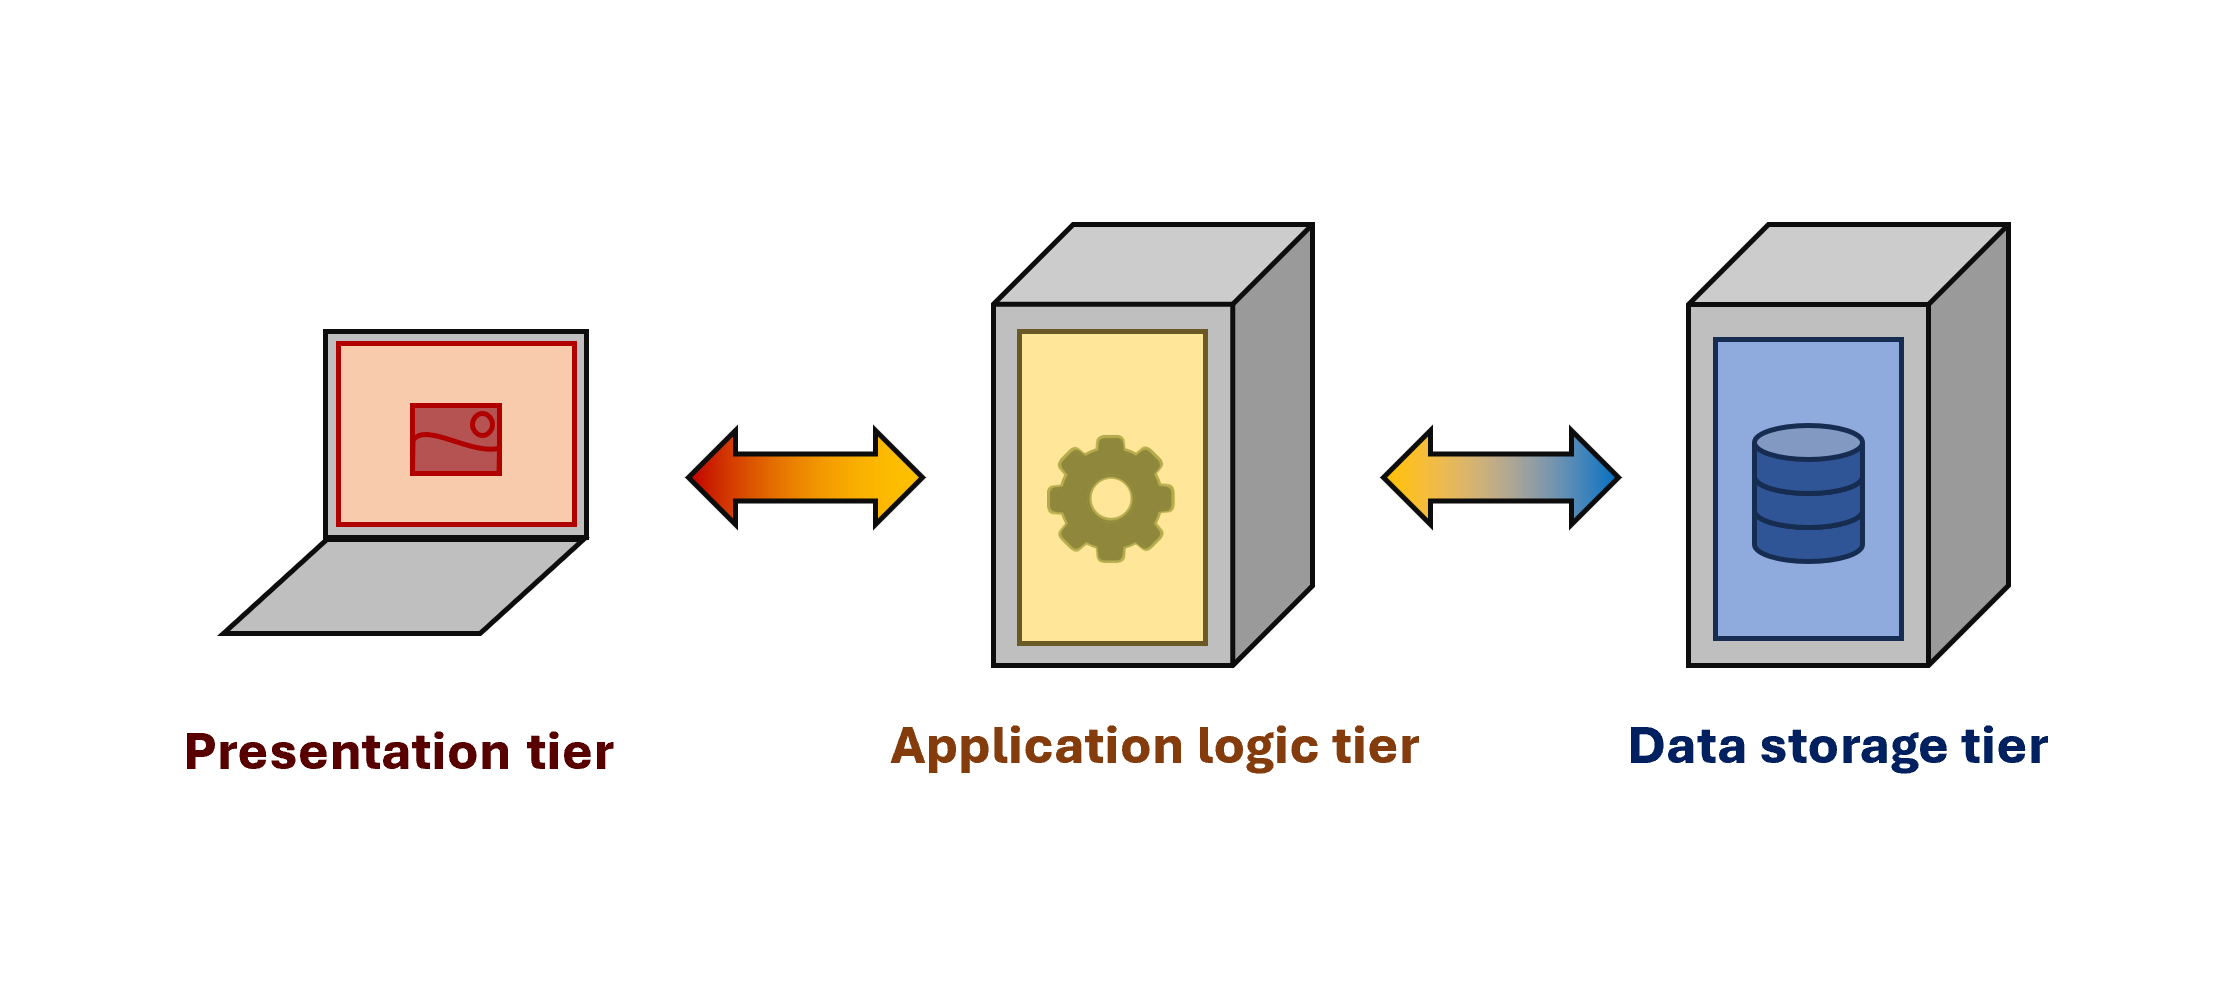
\includegraphics[width=0.9\linewidth]{Images/Threetiers.png}
    \caption{Visual representation of a three-tier architecture}
    \label{fig:enter-label}
\end{figure}

\begin{enumerate}
    \item \textbf{Presentation Tier:} its functions are providing the user interface, and handling user interactions. This tier is client side and interacts directly within users' browsers. All web-based interfaces are executed on the client-side, allowing educators and students to interact with the CKB platform. Since the computation is done locally on the client, the user experience will be efficient and responsive.
    \item \textbf{Application Logic Tier:} it’s positioned on the server-side, and its function is encapsulating the core functionalities of the CKB platform.  It contains the business logic, the code execution engines, facilitating communication between the users and the system. 
    \item \textbf{Data Storage Tier:} it's on server-side and it's the foundation of the architecture, where platform’s relational databases store, manage and retrieve all necessary information. To optimize data accessibility and ensure data integrity, a database management system (DBMS) is employed. For security measures, encrypted connections and access controls are implemented, to safeguard users’ sensitive information and system data, and against unauthorized access and data breaches.
\end{enumerate}
The CKB platform can be accessed only via web browser, which interacts with the presentation tier. On the server side there are two components situated in the application tier (application server and web server) and one component situated in the data tier (database server). The web server handles the HTTP requests sent by browsers and returns the correct web pages in response, it also need to communicate with the application server via suitable API calls if, to satisfy such requests are necessary some data from the database, this because the web server and the DB are not directly connected.\\
The application server communicates with the database server that retrieves all the information about students, educators, battles, tournaments, badges, deadlines and so on from the DB. This because the application tier must be able to add, delete or modify data in the data tier using API calls. \\
In addition, the application server also needs to communicate with an Email service provider, to send e-mails to users, and with the GitHub Action service via some API call, to provide the code written by teams to the system, which evaluates it and updates immediately the ranking.\\
In the end, the database server acts as an intermediary between the application server and the DBMS, managing connections, processing queries, and ensuring the overall efficiency and reliability of database operations. \\ \\
Since the system is distributed, so are the web servers, the application servers and the database servers, for this reason three load balancers are inserted into the architecture to dispatch the requests to web servers and application servers: all the requests coming from web browsers are captured by a load balancer that redirects the request to one of the web servers available to handle it. Then the web server manipulates the request and forwards it to the second load balancer, that dispatches requests from web servers to the application server that better elaborates the request in terms of time. \\ \\
The database should be clustered so that consistency is guaranteed, and the performances are sufficient to fulfill a large number of queries in a reasonable time. The replicated database servers' main function is to manage all data relevant to the application. The third load balancer is interposed between application servers and database servers. \\ \\
To guarantee a good level of security, a firewall is installed between every tier and between the external network (internet) and the internal network. Its functionalities are monitor, filter, and control incoming and outgoing network traffic based on predetermined and personalized security rules; it works as barriers between a trusted internal network and untrusted external networks that control the flow of traffic and prevent unauthorized access, protecting against various cyber threats and attacks. For other security measures, a Web Application Firewall (WAF) and an Intrusion Detection System (IDS) are integrated into the application tier, the first is necessary to safeguard against common web application threats and enhance overall security, while the second monitors and analyzes system activities, detecting and responding to suspicious behavior that may compromise the platform's integrity. \\ \\
In the following sections there is a presentation about the components of the systems and their interactions, completed with diagrams and schemes. Then, given the description of the components and their characteristics, an exhaustive discussion concerning the run time specifications of the system are presented with the use of sequence diagrams. Finally, a dependency analysis of the component interfaces is shown.

\newpage

\begin{figure}[H]
    \centering
    {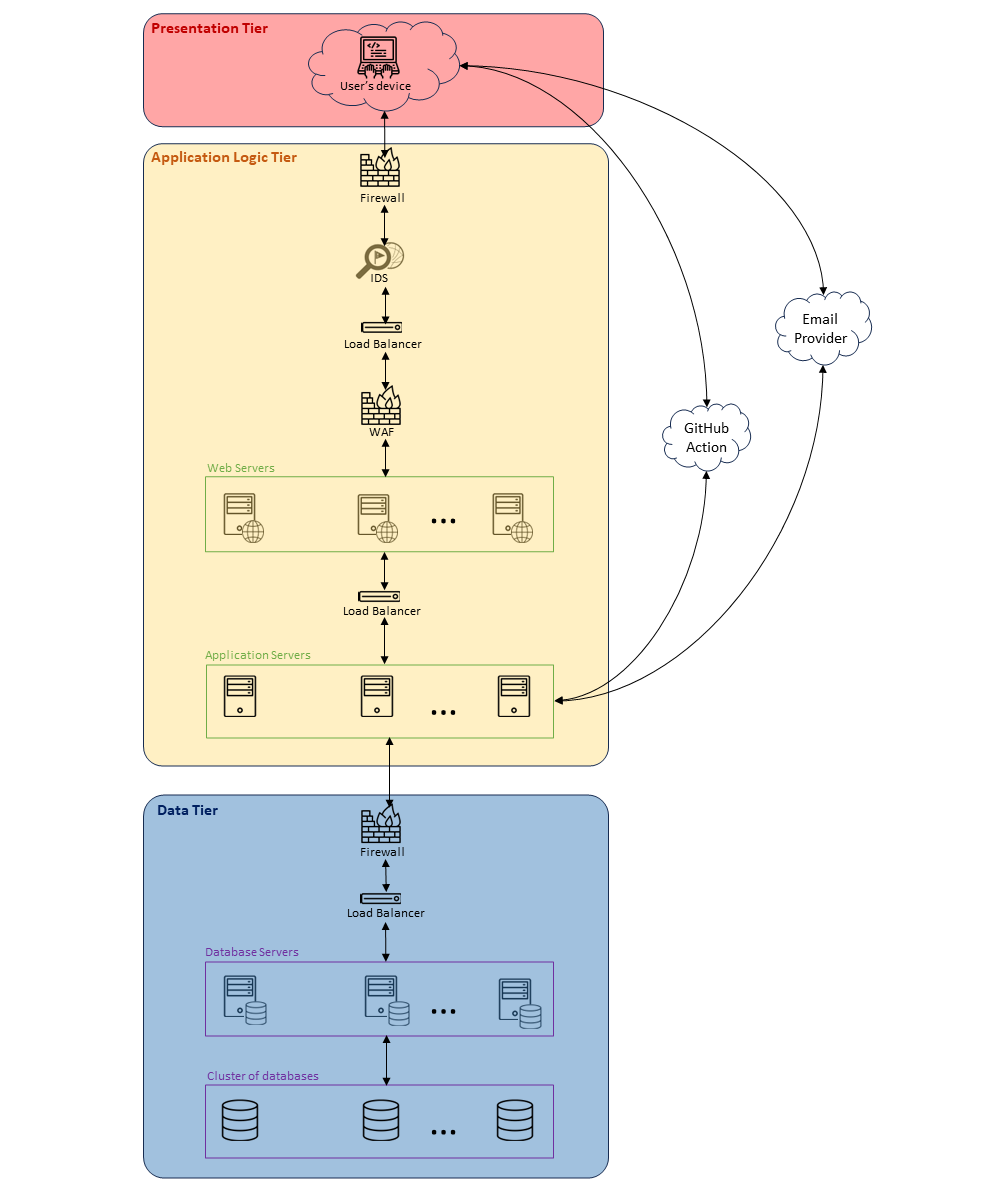
\includegraphics[width=1.2\linewidth]{Images/Architecture.png}}
    \caption{System Architecture}
    \label{fig:system_architecture}
\end{figure}

\newpage
 
\subsection{Component View}


\begin{figure}[H]
    \centering
    \rotatebox{-90}{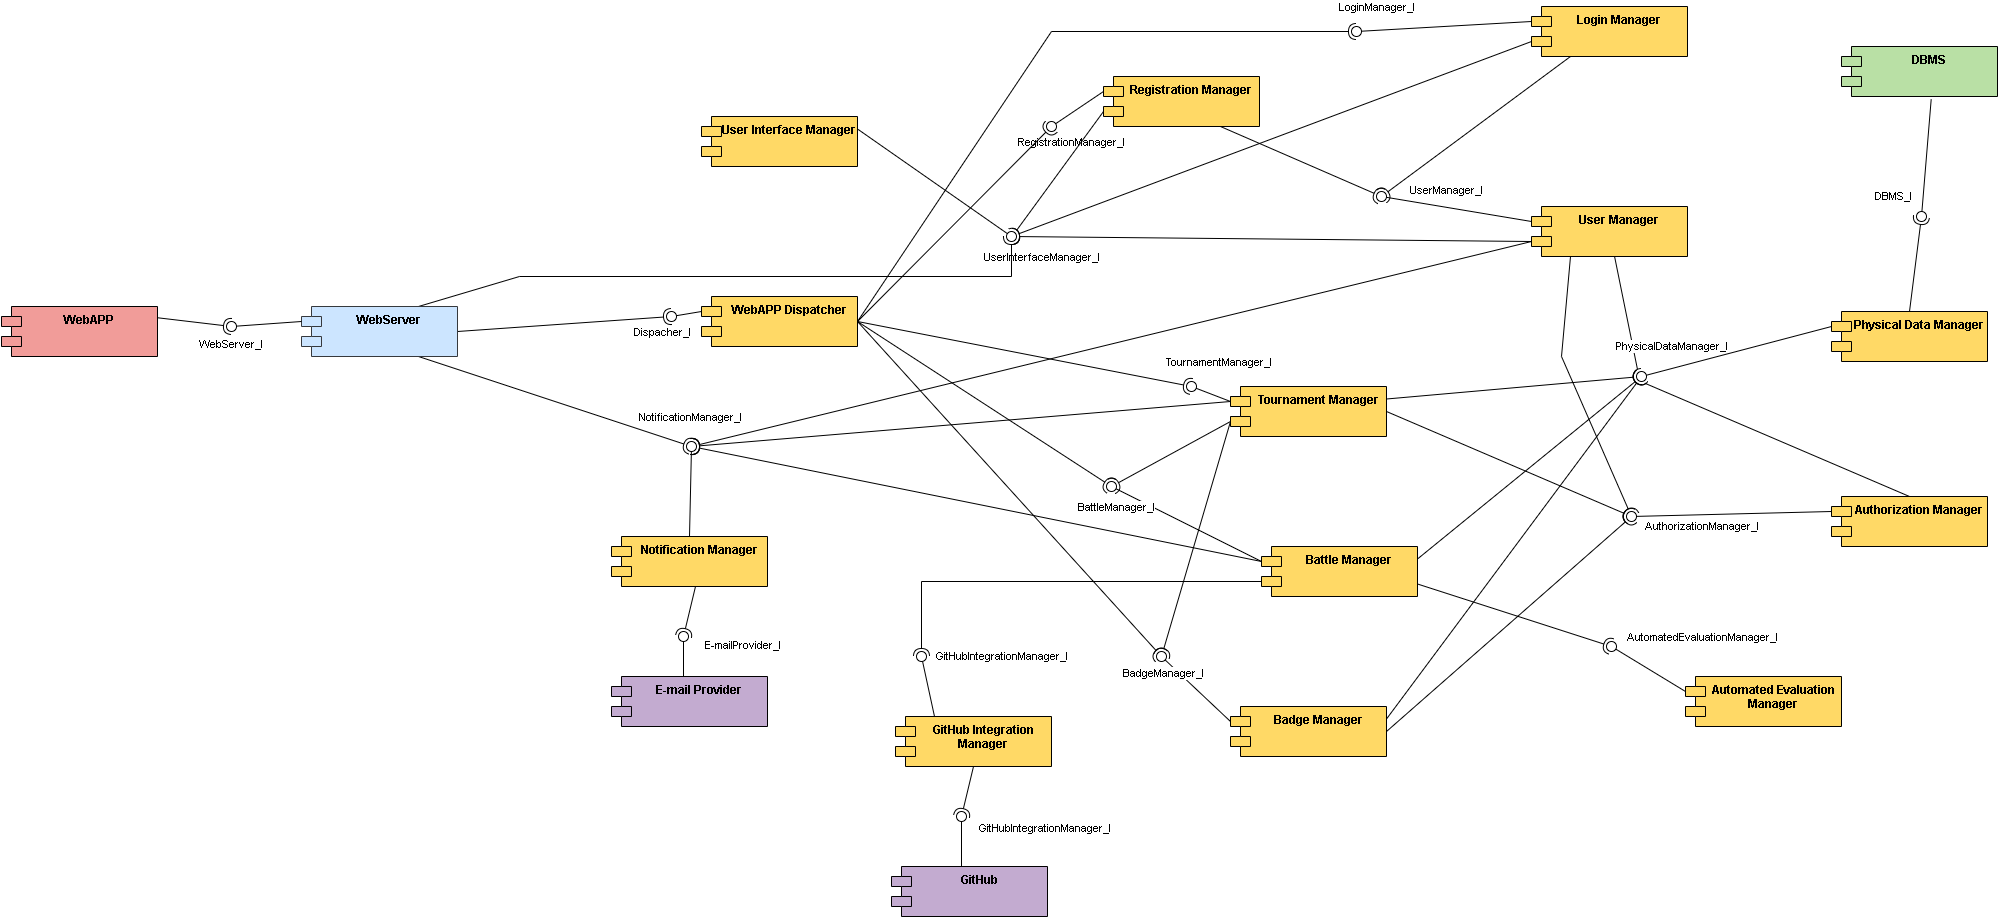
\includegraphics[width=1.35\linewidth]{Images/ComponentDiagram.png}}
    \caption{Component diagram}
    \label{fig:component_diagram}
\end{figure}

\begin{itemize}

    \item \textbf{Web App Dispatcher:} \\
    Handles the incoming requests, forwarding them to the correct component in order to subdivide the workload and correctly elaborate each request. Since all of the incoming requests need to be analyzed and dispatched to the correct manager, this component is replicated in the physical system in order to handle important loads of requests.

    \item \textbf{User Manager:} \\
    Handles students' and educators' data such as login parameters, profile description, badges, and more. When a new user is created, its data are collected from this component. When a user wants to log into the system, the User Manager collects the relevant data for the authentication of the user. When the profile of a student or an educator is required, this component's task is to retrieve all the required information about the requested user.

    \item \textbf{Registration Manager:} \\
    Handles user registration process. Checks the validity of the inserted data, imposing password complexity policies and preventing users from creating multiple accounts with the same information. If all the provided information is correct, it is stored in a secure manner.

    \item \textbf{Login Manager:} \\
    Handles user login and authentication processes, keeping track of unusual behaviors, and correctly handles sensitive data. The implementation of secure channels for the exchange of sensitive data even within the system is important to avoid data breaches: the Login Manager keeps this and all the other important security aspects into account.

    \item \textbf{Authorization Manager:} \\
    Handles user authorization processes.
    Manages user roles (Students, Educators) and their respective permissions. For example, when an educator wants to create a new battle within a tournament, this component checks whether permission has been granted from the creator of the tournament. When specific data about a user or about a battle are requested, the Authorization Manager ensures that the issuer is allowed to read the desired data.

    \item \textbf{Tournament Manager:}  \\
    Manages the creation, updating, and closure of tournaments. Includes components for handling registrations and scoring. Upon creation of a new tournament by an educator, the Tournament Manager handles all the necessary changes, providing continuously updated battles list and ranking. When a tournament is closed, the Tournament Manager maintains all the relevant information.

    \newpage

    \item \textbf{Battle Manager:}  \\
    Manages the creation, updating, and closure of battles.
    Includes components for handling registrations, submissions, and scoring.
    When a new battle is created, the Battle Manager keeps track of the registration issued by the student, and once the battle starts it works synergistically with the GitHub Integration Manager and Automated Evaluation Manager to provide a real-time experience to the user. Once the battle closes, the Battle Manager awaits the educator's evaluations if necessary, providing all the relevant information to the Tournament Manager once the final ranking has been established.

    \item \textbf{GitHub Integration Manager:} \\
    Facilitates the integration with GitHub for repository creation, forking, and workflow setup.
    Manages the communication between the CKB platform and GitHub.

    \item \textbf{Automated Evaluation Manager:}\\
    This component handles the ongoing evaluation of student submissions using build automation and testing tools. This component is designated to provide a real-time evaluation of student solutions to create a continuously updated battle rank. If the educator of the battle chooses not to manually evaluate final submissions, once the battle closes this component automatically evaluates the last solution issued by each team.

    \item \textbf{User Interface (UI) Manager:} \\
    Responsible for presenting information to users and capturing their interactions. Includes components for displaying tournament and battle information, user profiles, and submission interfaces. This component is instantiated in order to be able to implement new features inside the user interface without the need of structural changes in the system. 

    \item \textbf{Badge Manager:} \\
    Manages the creation and assignment of badges within the context of tournaments.
    Handles the association of badges with specific rules and user achievements.
    When a tournament is closed, the tool checks the eligibility of each student registered to the tournament, collecting data from all the battles created within the tournament and assigning each badge to deserving students.
    
    \item \textbf{Notification Manager:} \\
    Manages the generation and delivery of notifications to users about new tournaments, battles, and closures. Notifications can be either visualized on the web app or sent via email to the users.
    
    \item \textbf{Physical Data Manager:} \\
    Stores and retrieves data related to users, tournaments, battles, submissions, and other relevant information. It is responsible for the communication with the DBMS, handling the topology of distributed and replicated databases, keeping track of the accesses and modifications performed by different processes for maintainability and security reasons.

\end{itemize}


\subsection {Deployment View}

\begin{figure}[H]
    \centering
    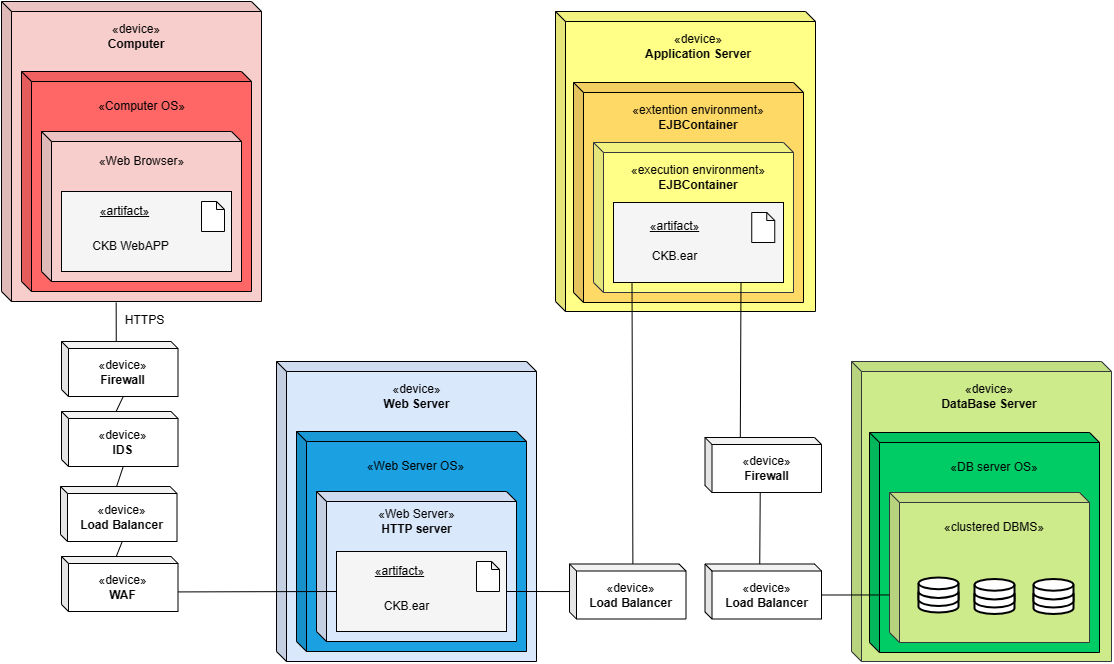
\includegraphics[width=1\linewidth]{Images/DeploymentView.png}
    \caption{Deployment view of the system}
    \label{fig:enter-label}
\end{figure}

\begin{itemize}
    \item \textbf{Client devices (Computers with web browsers):} \\
    The physical device required to access the CKB platform is a computer with the capability of connecting to the internet. No specific applications have to be installed on the device in order to access the platform apart from a generic web browser, required for navigating the web and reaching the CKB web page.
    \item \textbf{Firewall:} \\
    It acts as a crucial line of defense for a network, employing a range of functionalities to safeguard against potential threats and unauthorized access, monitoring all incoming and outgoing network traffic within the system, distinguishing between harmless data and potentially harmful elements. It acts as a gatekeeper, checking all data packets based on a set of predetermined or personalized security rules: it evaluates the characteristics of each packet, such as source and destination addresses, port numbers, and protocol types. By doing so, it makes informed decisions about whether to permit or deny passage to specific packets and so works as a barrier between the trusted internal network and the untrusted external networks. It’s positioned between every tier, this strategic positioning allows the firewall to exercise control over the flow of traffic, ensuring that only legitimate and authorized packets pass through. In addition, it establishes a secure perimeter around the internal network, actively managing the access permissions. It acts as a shield against various cyber threats, including malware, phishing attacks, and intrusion attempts.

    \item \textbf{Intrusion Detection System (IDS):} \\
    It’s a fundamental component in cybersecurity, designed to provide continuous monitoring, analysis, and response to safeguard the integrity of a platform. Its primary function is to actively monitor and analyze system activities, controlling users’ behavior, applications, and network traffic in real-time, with the goal to identify any deviations from established patterns that could signal potential security threats or unauthorized accesses. The monitoring is done through the observation of data sources such as network traffic logs, system logs, user activities, and application behaviors, aggregating and correlating data from these sources. It also gains a comprehensive knowledge of the typical patterns of operation of the system. \\
    The analysis phase employs advanced algorithms to detect anomalies or patterns indicative of malicious activities: it compares the observed behavior against predefined profiles of normal or acceptable behavior, and any deviation triggers an alert, signaling potential security incidents. \\
    It is also equipped with responsive capabilities, in fact after detecting suspicious behavior, it initiates appropriate responses to mitigate the threat. These responses can go from generating notifications for further investigation to taking immediate action to block or quarantine malicious entities.

    \item \textbf{Load Balancer:} \\
    Its function is to distribute tasks and requests efficiently across multiple servers to optimize resource utilization, enhance performance maximizing the utilization of computing resources, and ensure high availability. This distribution is done in a way that prevents any single server from becoming overloaded, to prevent performance degradation or potential system downtime. It evenly distributes not just processing loads, but also memory usage, and network bandwidth among the servers. It also regularly monitors the health and status of individual servers and helps with system’s availability by directing traffic away from servers that may have issues or are temporarily unavailable, directing traffic to healthy servers, ensuring uninterrupted service for users. It also facilitates horizontal scaling by efficiently adding or removing servers from the system. 
    
    \item \textbf{Web Application Firewall (WAF):} \\
    It is an important component within the system's security infrastructure, its purpose is to provide defense against a wide range of common web application threats, vulnerabilities, and attacks, safeguarding the integrity, confidentiality, and availability of user data and system resources. It is designed to identify, analyze, and mitigate common web application attacks such as SQL injection, cross-site scripting (XSS), cross-site request forgery (CSRF), and other injection-based vulnerabilities, performing real-time analysis of HTTP requests and responses and identifying patterns indicative of potential threats, it prevents malicious users from exploiting vulnerabilities in the platform. Network administrators adjust rules and policies dynamically, such as specifying what type of requests are allowed or denied and customizing the security strength of the system. To prevent unauthorized access and data leakage, it controls incoming and outgoing traffic for sensitive information such as personal information and other confidential data, and it also can mask, block, or log sensitive data to maintain confidentiality. Another important function is the safeguarding of user sessions by detecting and preventing session-related attacks that could be employed to compromise user sessions and access unauthorized areas of the platform. Finally, it generates logs and reports that can be valuable to demonstrate platform's adherence to security best practices.
    
    \item \textbf{Web Server:} \\
    It's part of system's architecture, responsible for managing the communication between clients (browsers) and the application server, it has a fundamental role in receiving and handling HTTP requests initiated by users' browsers, ensuring the correct delivery of web pages, in fact it works as the entry point within the platform. To provide dynamic content and fulfill user requests that require data from the database, it communicates with the application server via API calls, ensuring that served web pages are up-to-date and reflect the most recent information stored in the system: it acts as an intermediary between the client-side and back-end components such as the database, abstracting the complexities of back-end operations and preventing direct connections, enhancing security and modularity within the system. It also implements caching strategies to optimize content delivery, in fact frequently accessed static content can be cached to reduce latency and increase the responsiveness of the platform.
    
    \item \textbf{Application Server:} \\
    It works as the core computational engine of the system and is responsible for executing business logic, managing data flow, and facilitating communication between various components, ensuring the dynamic and responsive functioning of the system. One of its primary responsibilities is to communicate with the database server through API calls for retrieving, adding, deleting, or modifying data stored in the database, ensuring dynamic updates, and maintaining data integrity. It also communicates with third-party tools and services through API calls. 
    
    \item \textbf{Database Server:} \\
    It is an intermediary between the application server and the Database Management System (DBMS). This component manages and optimizes interactions with the underlying database, providing an efficient data storage and retrieval process. It handles the establishment, maintenance, and termination of connections, ensuring that the application server can communicate with the database securely and reliably. It acts as a gateway for queries: it processes SQL queries received from the application server and optimizes them, enhancing the overall performance. It also implements concurrency control mechanisms, since multiple requests may occur simultaneously, ensuring that transactions are executed in a controlled manner, preventing conflicts, and maintaining the consistency of the database. In addition, it enforces data integrity constraints defined in the database schema: it validates incoming data to prevent inconsistencies and errors in the stored information. It has a caching mechanism to store frequently accessed data temporarily to reduce latency and improve response times. Finally, it facilitates the creation of database backups at regular intervals and assists restoring data in the event of data loss or corruption.
\end{itemize}

\subsection{Runtime View}
 The following sequence diagrams represent the runtime view of the system applied to the most important use cases. The purpose of these diagrams is to illustrate the interaction between the components described in the previous sections: for the precise details about the interfaces offered by each component, refer to the next section.

 \begin{itemize}
    \item \textbf{Student Registration:}

    \begin{figure}[H]
        \centering
        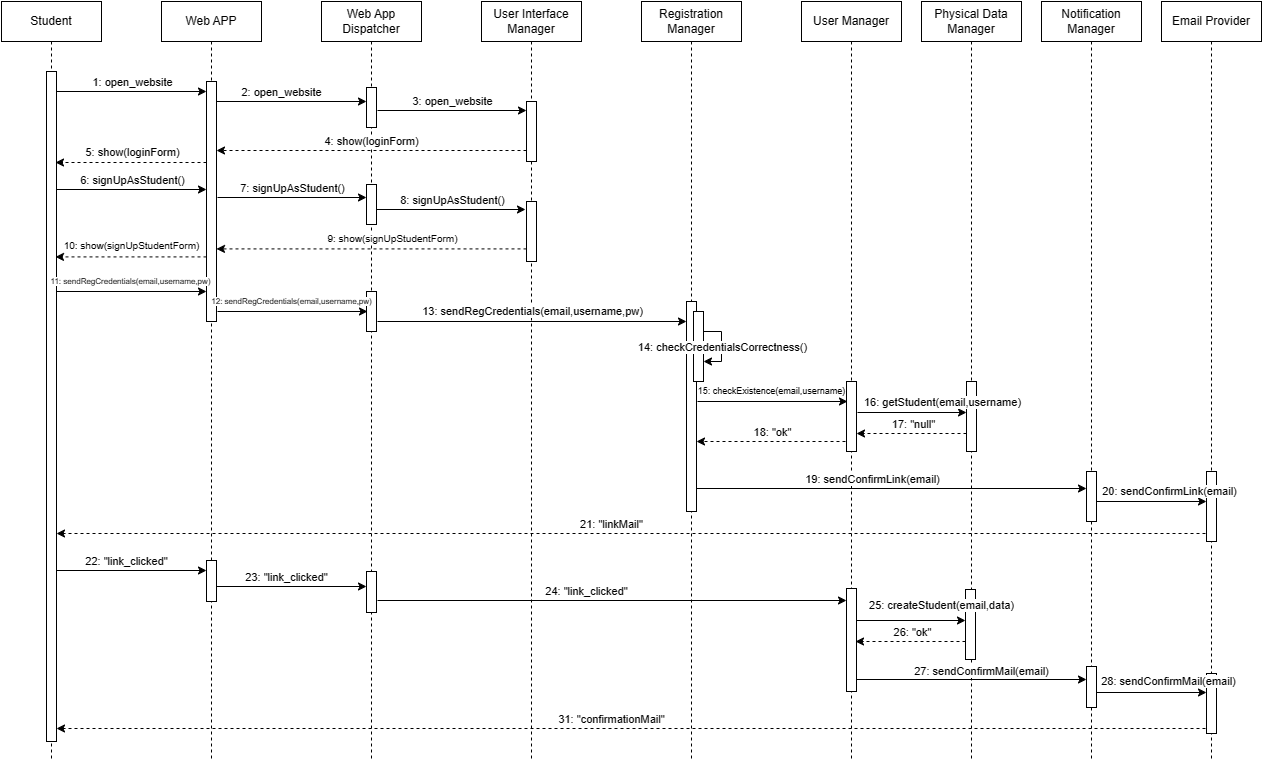
\includegraphics[width=1\linewidth]{Images/RV1.png}
        \caption{Student registration runtime view}
        \label{fig:rv1}
    \end{figure}

    This sequence diagram shows all the actions performed when a student registers to the system. When the "sign up as student" page has been created by the User Interface Manager and shown to the student via the Web Application, the student inserts their credentials and sends them to the Registration Manager. The Registration Manager checks the correctness of the incoming data, such as the validity of the email or the length of the password, and then queries the User Manager to check if another student with the same credential exists. When the validity of the data has been assessed, an email containing the confirmation link is sent to the submitted email address. When the link is clicked, the system confirms the insertion of the new student, and a final email is sent to the user.

    \item \textbf{Educator Registration:}

    \begin{figure}[H]
        \centering
        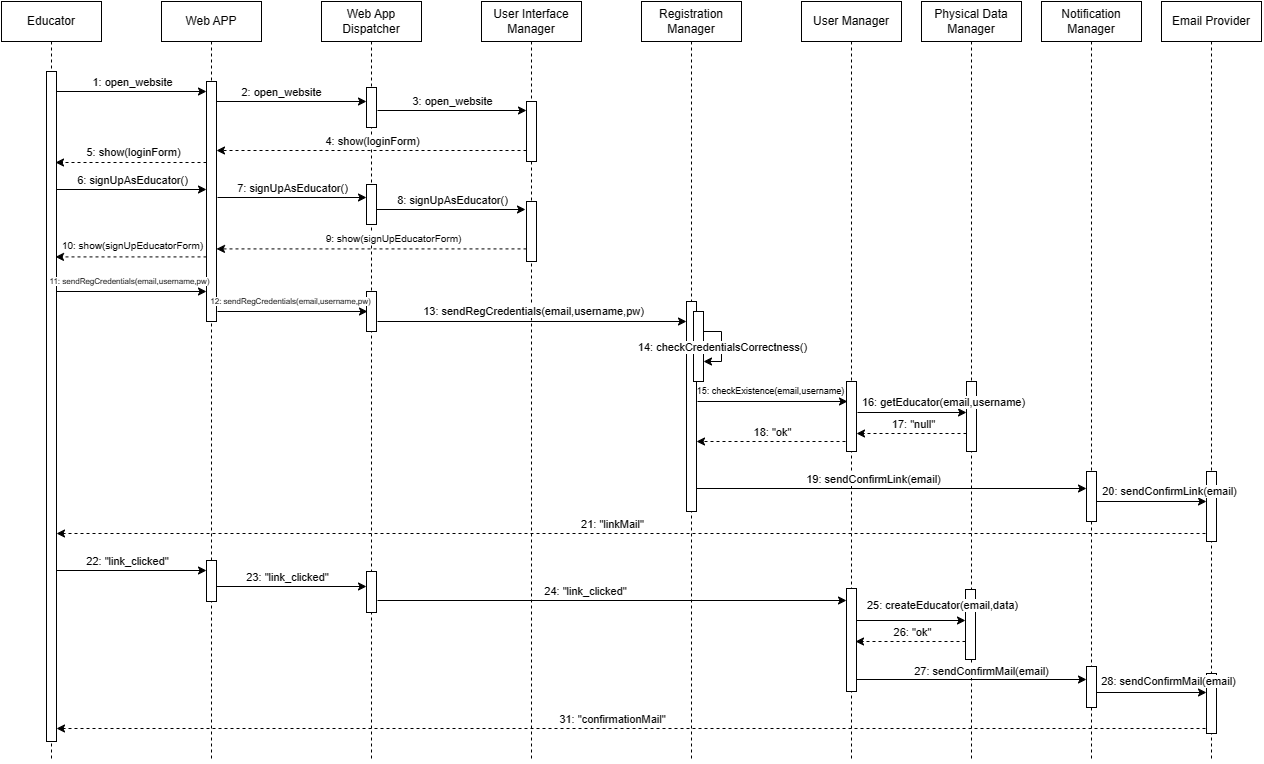
\includegraphics[width=1\linewidth]{Images/RV2.png}
        \caption{Educator registration runtime view}
        \label{fig:rv2}
    \end{figure}

    This sequence diagram shows all the actions performed when an educator registers to the system. When the "sign up as educator" page has been created by the User Interface Manager and shown to the educator via the Web Application, the educator inserts their credentials and sends them to the Registration Manager. The Registration Manager checks the correctness of the incoming data, such as the validity of the email or the length of the password, and then queries the User Manager to check if another educator with the same credential exists. When the validity of the data has been assessed, an email containing the confirmation link is sent to the submitted email address. When the link is clicked, the system confirms the insertion of the new educator, and a final email is sent to the user.

    \newpage
    
    \item \textbf{Student Login:}

    \begin{figure}[H]
        \centering
        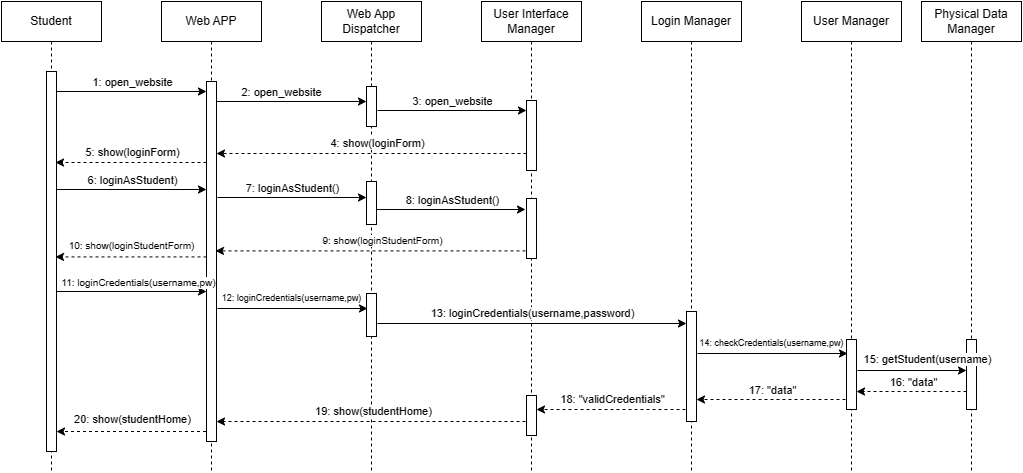
\includegraphics[width=1\linewidth]{Images/RV3.png}
        \caption{Student login runtime view}
        \label{fig:rv3}
    \end{figure}

    This sequence diagram shows all the actions performed when a student logs into the system. Once the student has selected "login as student", its credentials are sent to the Login Manager, which is responsible for querying the User Manager, collecting the data regarding the student corresponding to the inserted credentials and checking whether the authentication data are correct. If the check is positive, the User Interface prepares the home page, which is displayed by the Web Application to indicate the correct access to the profile.

    \newpage

    \item \textbf{Educator Login:}

    \begin{figure}[H]
        \centering
        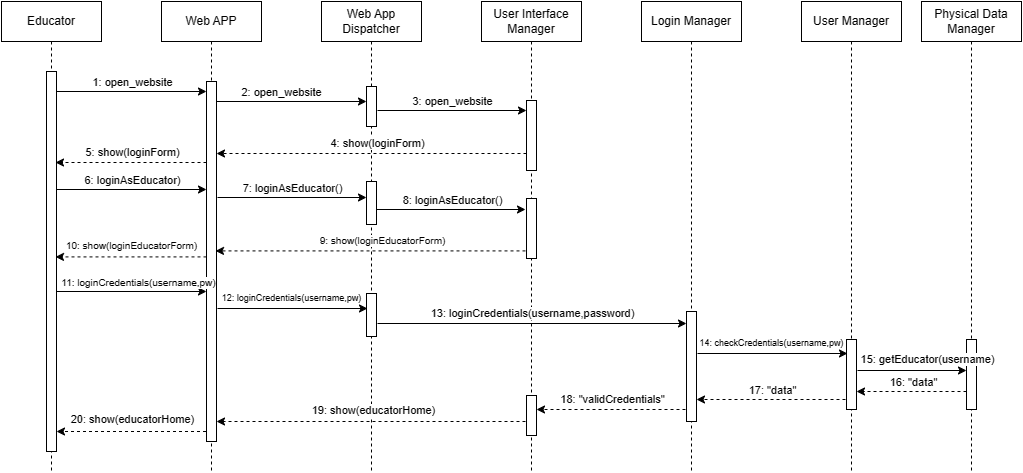
\includegraphics[width=1\linewidth]{Images/RV4.png}
        \caption{Educator login runtime view}
        \label{fig:rv4}
    \end{figure}

    This sequence diagram shows all the actions performed when an educator logs into the system. Once the educator has selected "login as educator", its credentials are sent to the Login Manager, which is responsible for querying the User Manager, collecting the data regarding the educator corresponding to the inserted credentials and checking whether the authentication data are correct. If the check is positive, the User Interface prepares the home page, which is displayed by the Web Application to indicate the correct access to the profile.

    \newpage
    
    \item \textbf{Tournament Creation:}

    \begin{figure}[H]
        \centering
        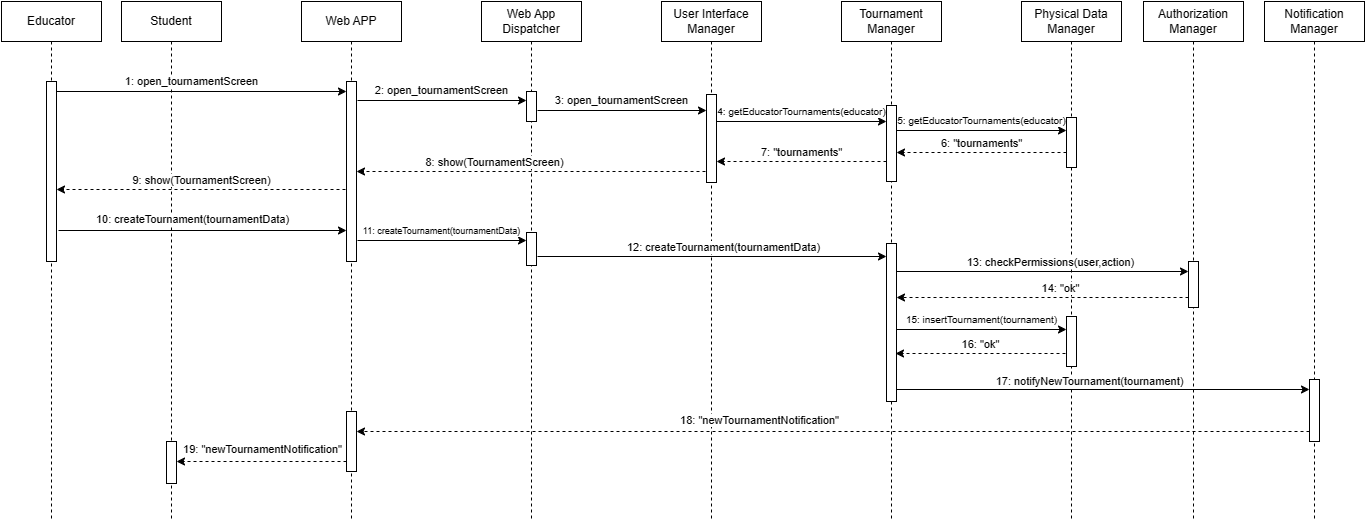
\includegraphics[width=1\linewidth]{Images/RV5.png}
        \caption{Tournament creation runtime view}
        \label{fig:rv5}
    \end{figure}

    This sequence diagram shows all the actions performed when an educator creates a new tournament. When the "tournaments" page has been displayed, the educator inserts all the required data for the creation of the tournament. When the educator confirms the action, the tournament's data is sent to the Tournament Manager. After a check by the Authorization Manager (to ensure that the user has permission to perform this action), the tournament is inserted into the database by the Physical Data Manager and a notification is sent to all the students.

    \newpage
    
    \item \textbf{Add Battle Permission Granting:}

    \begin{figure}[H]
        \centering
        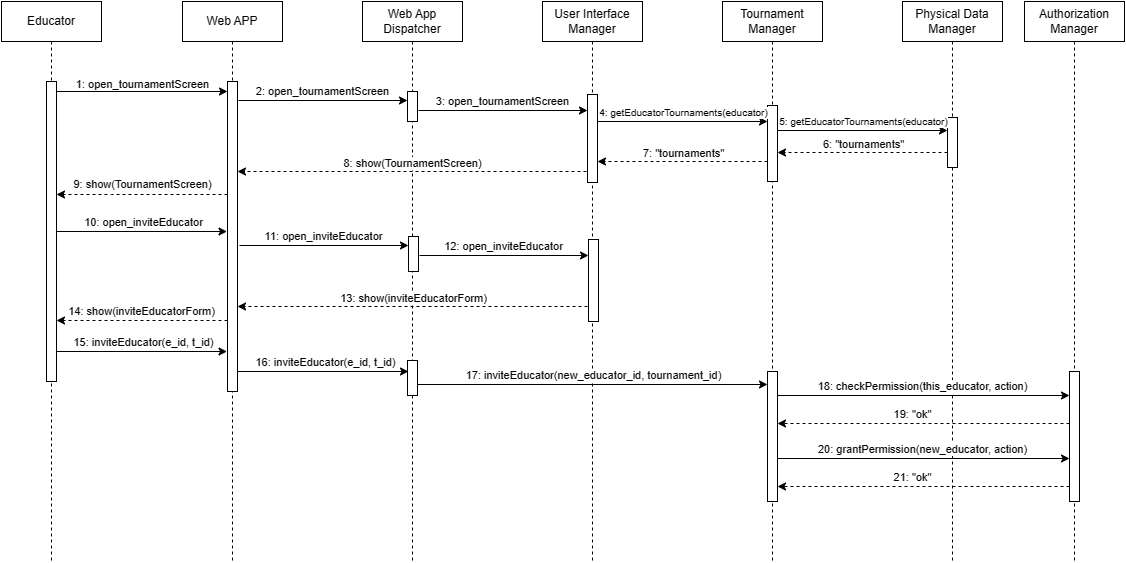
\includegraphics[width=1\linewidth]{Images/RV6.png}
        \caption{Add battle permission granting runtime view}
        \label{fig:rv6}
    \end{figure}

    This sequence diagram shows all the actions performed when an educator grants another educator the permission to create battles within a tournament. When the designated form has been displayed, the educator insert the other educator's id (either the username or the email address), which is then sent to the Tournament Manager. The Tournament Manager first checks if the issuer of the request has the granting permission and then signals the Authorization Manager that a new educator can create battles within the specific tournament.

    \newpage

    \item \textbf{Battle Creation:}

    \begin{figure}[H]
        \centering
        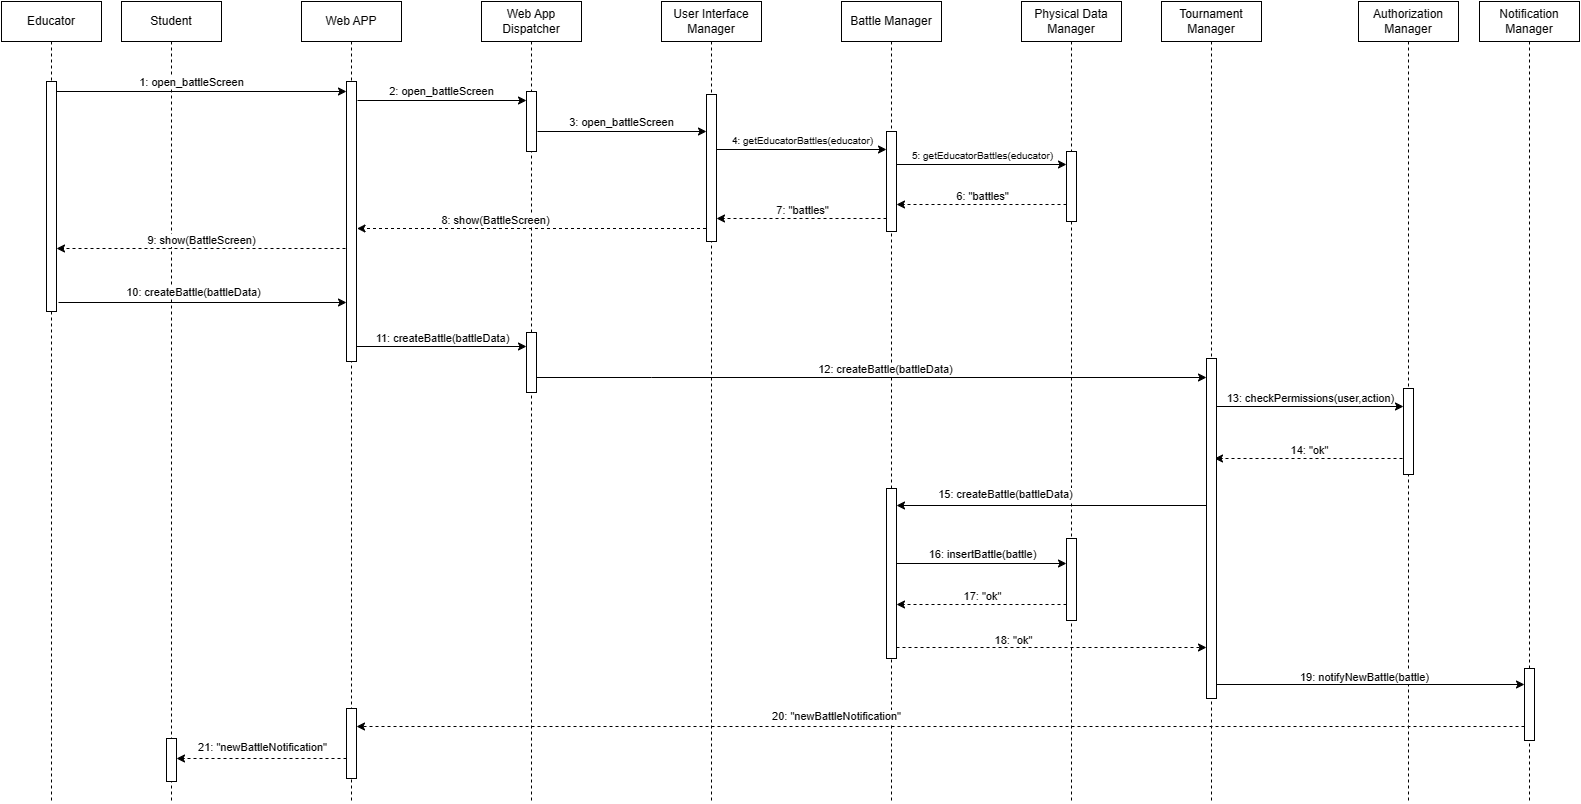
\includegraphics[width=1\linewidth]{Images/RV7.png}
        \caption{Battle creation runtime view}
        \label{fig:rv7}
    \end{figure}

    This sequence diagram shows all the actions performed when an educator creates a new battle. From the "battles" page, the educator submits all the battle's data, such as name, description, software components, automated evaluation settings, and so on. This information is then forwarded to the Tournament Manager. The Tournament Manager checks, via the Authorization Manager, if the educator has permission to create a new battle in the context of the specific tournament, and then triggers the creation of the battle via the Battle Manager. Finally, it sends a notification to all the students subscribed to the tournament.

    \newpage

    \item \textbf{Tournament Subscription:}

    \begin{figure}[H]
        \centering
        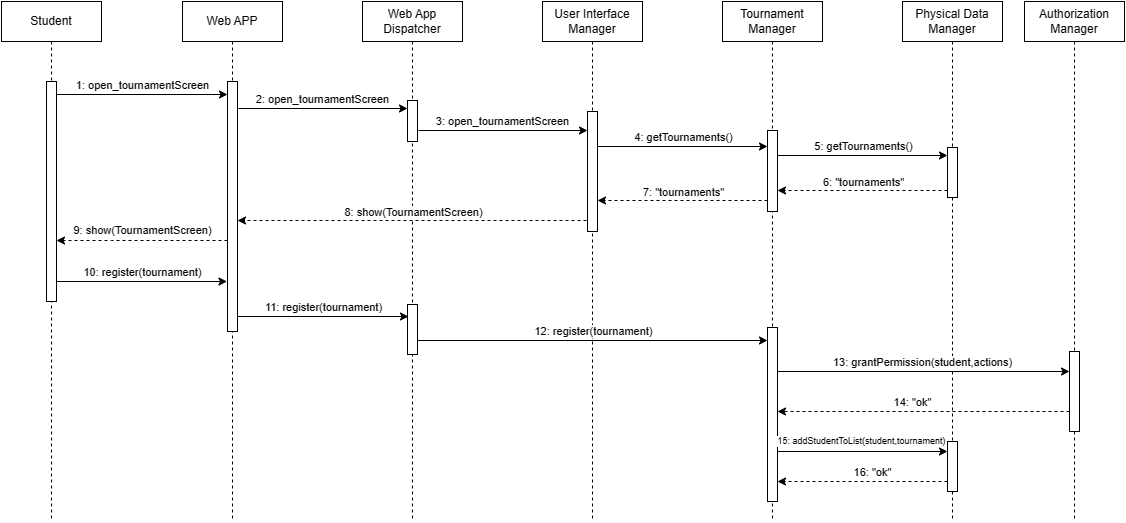
\includegraphics[width=1\linewidth]{Images/RV8.png}
        \caption{Tournament subscription runtime view}
        \label{fig:rv8}
    \end{figure}

    This sequence diagram shows all the actions performed when a student subscribes to a tournament. After the "tournaments" page has been displayed, the student select the tournament he wants to subscribe to. The request is forwarded from the Web App Dispatcher to the Tournament Manager, which is responsible for adding the permission to enlist for battle within the tournament to the student. The student is then added to the tournament student's list.

    \newpage

    \item \textbf{Team Formation:}

    \begin{figure}[H]
        \centering
        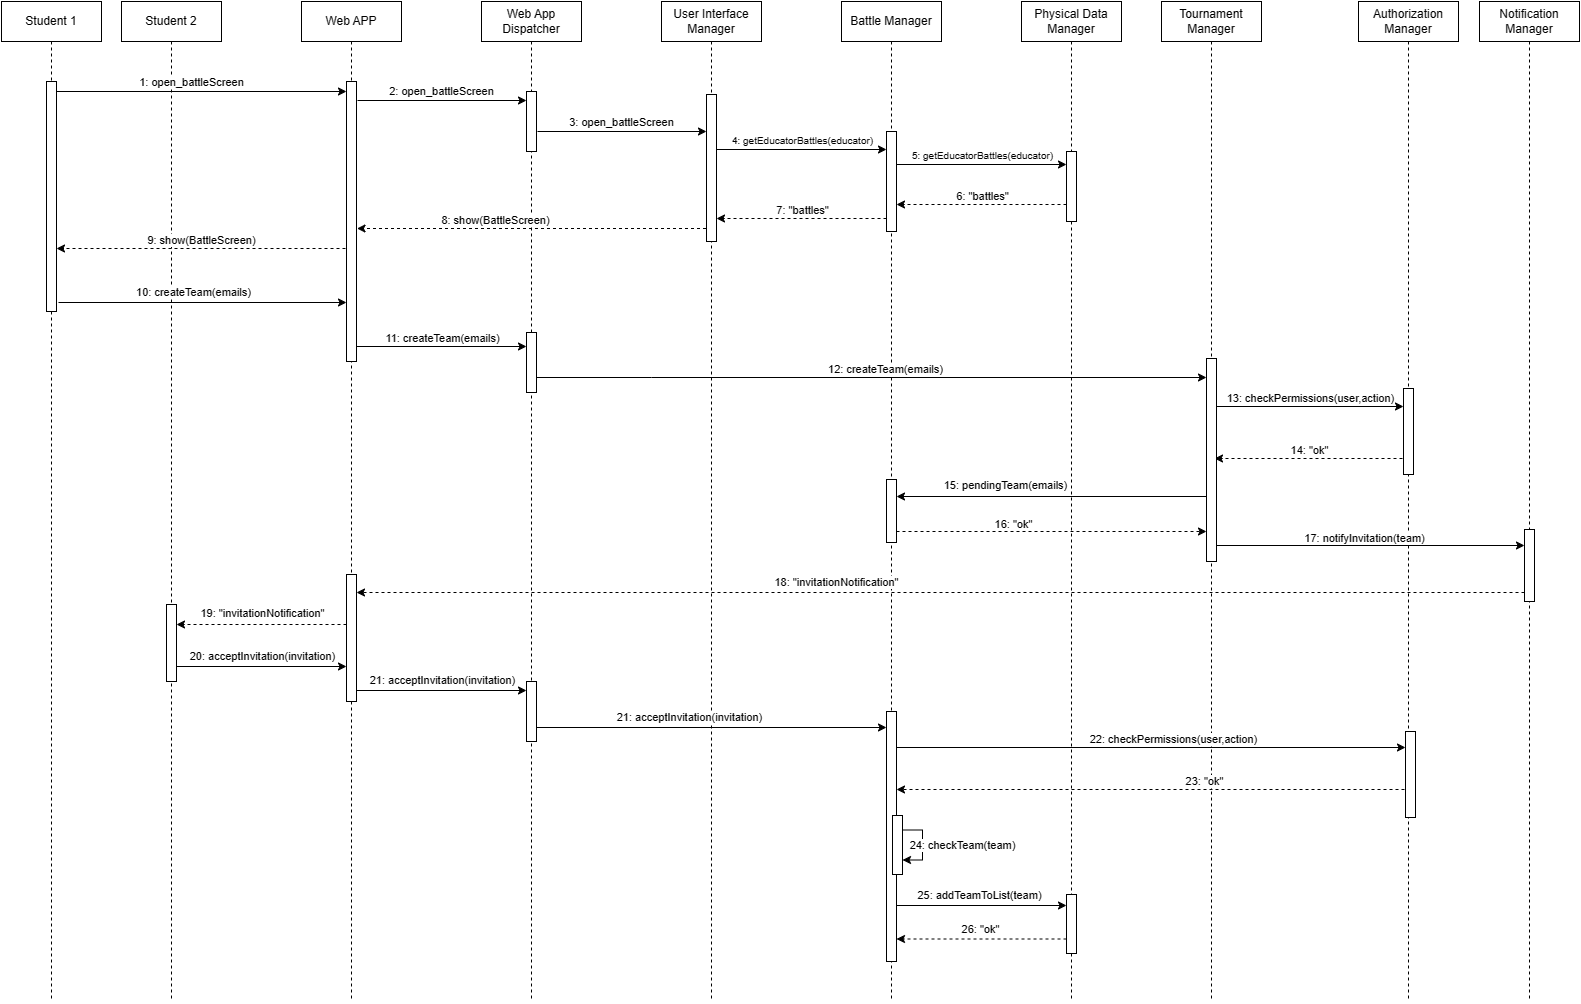
\includegraphics[width=1\linewidth]{Images/RV9.png}
        \caption{Team formation runtime view}
        \label{fig:rv9}
    \end{figure}

    This sequence diagram shows all the actions performed when a student wants to form a team to compete in a battle. The diagram includes both the team formation and the invitation handling. The student who wants to create the team selects the battle in the "battle" page, inserting the emails (or usernames) of their teammates. The request is sent to the Tournament Manager, which is responsible to check whether all the students in the team have permission to join the battle (for example, the student must be subscribed to the tournament). If the checks are positive, the team's information are forwarded to the Battle Manager and a notification is sent to the other teammates. When enough teammates accept the invitation, the Battle Manager inserts the team into the list of enlisted groups. If the group is formed by one student, and the battle allows single students to participate, no invitations are sent and the student is directly enlisted to the battle.

    \newpage

    \item \textbf{Continuous Integration:}

    \begin{figure}[H]
        \centering
        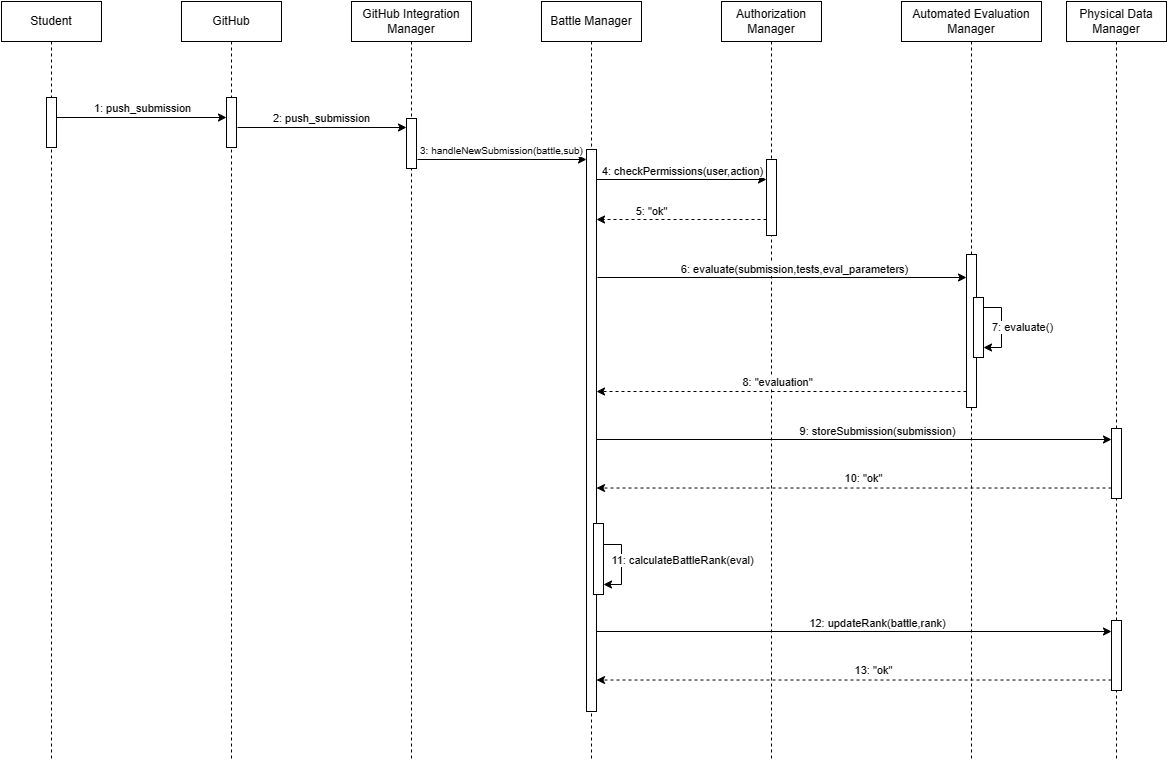
\includegraphics[width=1\linewidth]{Images/RV12.png}
        \caption{Continuous integration runtime view}
        \label{fig:rv12}
    \end{figure}

    This sequence diagram shows all the actions performed when a student submits a new solution for the Code Kata. Since no direct interaction happens between the student and the system, this runtime view does not correspond to any use case, but it is useful to display what happens during the battle. When the student performs a "push", via GitHub Action the submission is notified to the GitHub Integration Manager. The solution is then forwarded to the Battle Manager, which is responsible for checking if the issuer has permission to submit a new solution. Once the check has been performed, the student's code is sent to the Automated Evaluation Manager, which evaluates the solution based on the test cases and on the evaluation parameters provided by the educator at battle creation time. Finally, the solution is stored in the database and the battle rank is updated.

    \newpage

    \item \textbf{Real-time battle rank visualization:}

    \begin{figure}[H]
        \centering
        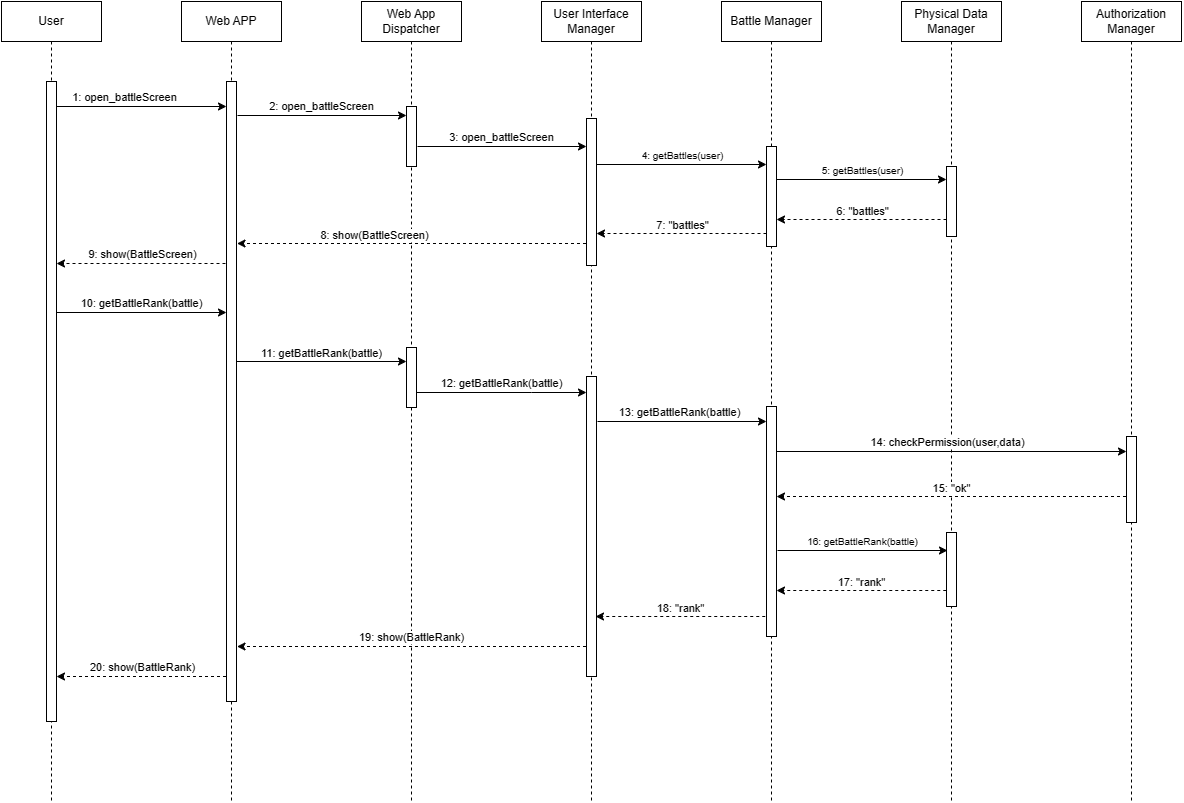
\includegraphics[width=1\linewidth]{Images/RV13.png}
        \caption{Real-time Battle Rank Visualization runtime view}
        \label{fig:rv13}
    \end{figure}

    This sequence diagram shows all the actions performed when and user (either a student or an educator), requests the current rank of a battle. Once the "battles" page has been displayed, the user selects the battle whose rank they are interested in. The request is forwarded to the User Interface Manager, that is responsible for collecting the data to be displayed. When the Battle Manager is consulted, after checking that the user has permission to access the data (in order to see the battle's rank, the user must be involved in a battle, either as the creator or as a participant), it queries the Physical Data Manager, returning the requested ranking to the User Interface Manager, that finally loads the rank page to show to the user.

    \newpage

    \item \textbf{Code Manual Evaluation and Rank Calculation:}

    \begin{figure}[H]
        \centering
        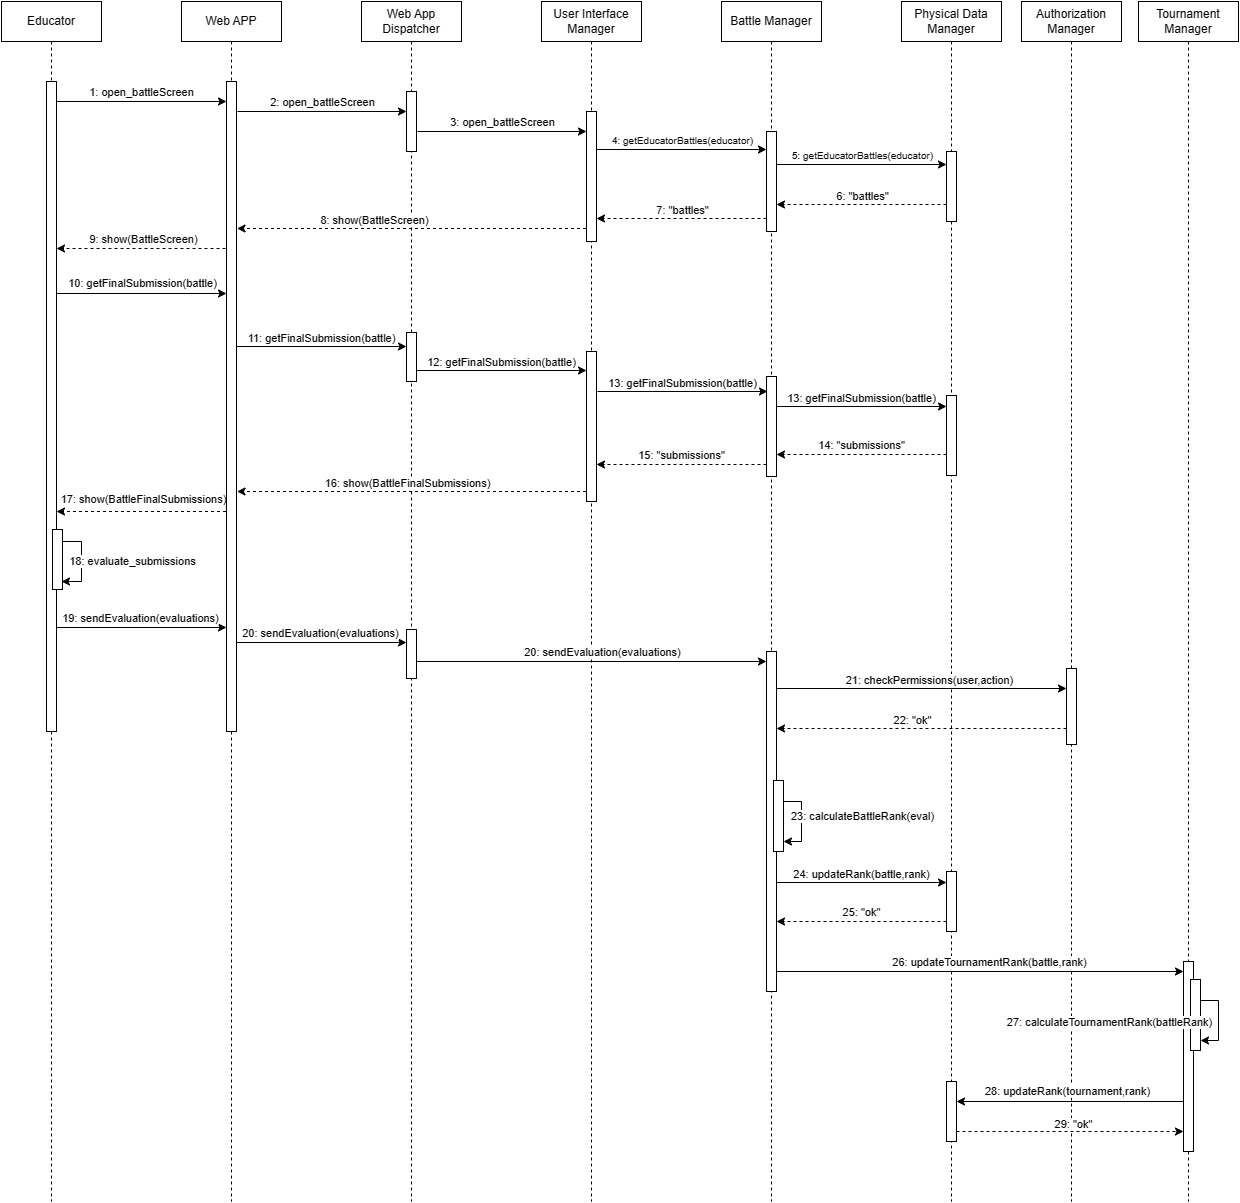
\includegraphics[width=1\linewidth]{Images/RV10.png}
        \caption{Code manual evaluation and Rank calculation runtime view}
        \label{fig:rv10}
    \end{figure}

    This sequence diagram shows all the actions performed when an educator evaluates the students' solutions after a battle has been closed. The educator collects all the teams' final submissions via the "battles" page. Once the submissions have been graded, the evaluations are sent to the Battle Manager. After an authorization check, the final battle ranking is calculated and stored in the database. The rank is then sent to the Tournament Manager, which is responsible for updating the rank of the tournament corresponding to the close battle.\\
    The runtime view in the case where the manual evaluation is not required is a simplified version of this one: when the battle is closed, the Battle Manager collects the evaluations from the Automated Evaluation Manager, proceeding then from step 23 with the calculation of the battle rank.

    \newpage

    \item \textbf{Tournament Rank Visualization:}

    \begin{figure}[H]
        \centering
        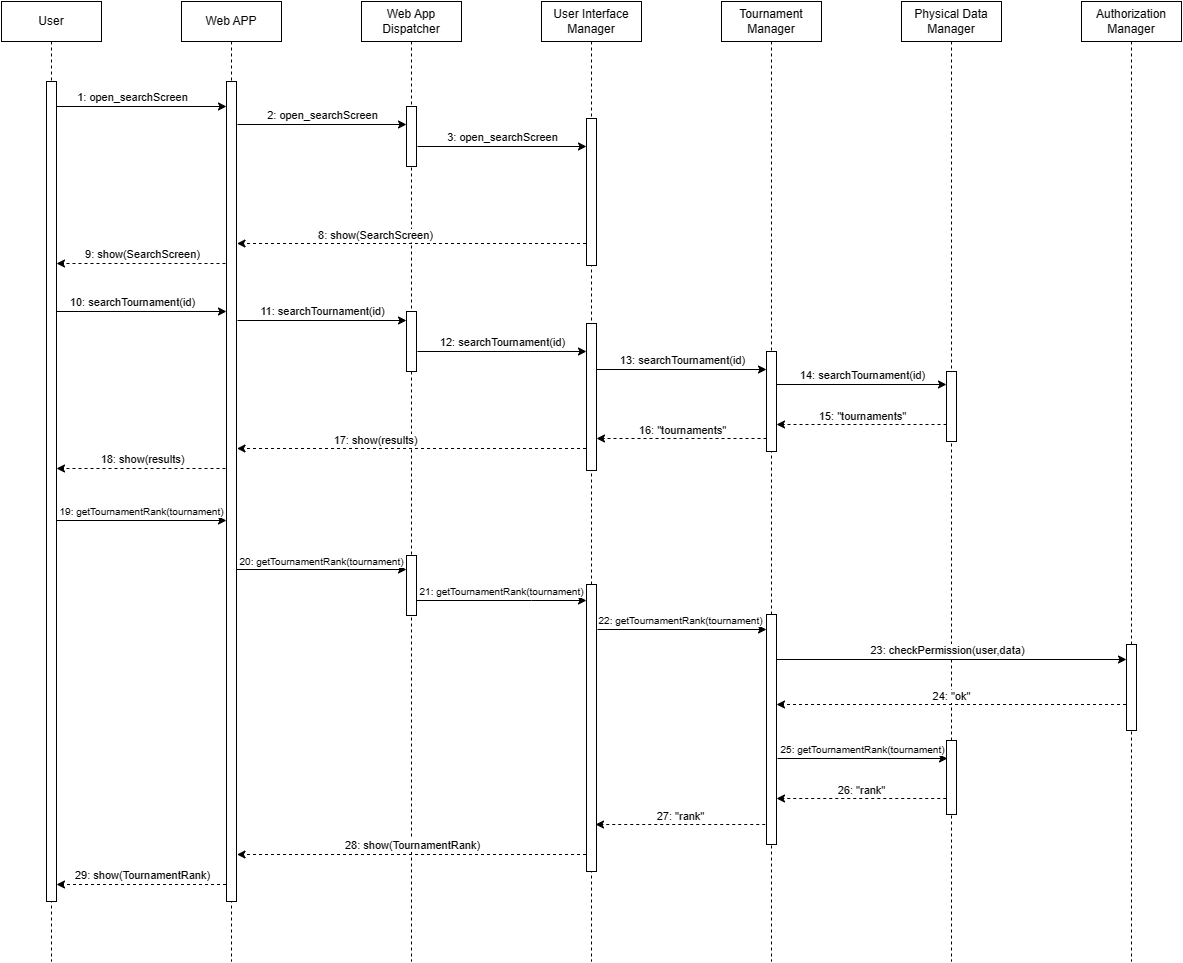
\includegraphics[width=1\linewidth]{Images/RV14.png}
        \caption{Tournament Rank Visualization runtime view}
        \label{fig:rv14}
    \end{figure}

    This sequence diagram shows all the actions performed when and user (either a student or an educator), requests the current rank of a tournament. In order to be able to see the rank of all ongoing or closed tournaments, the user first enters the "search" page. From there, the user insert an identification of the requested tournament (i.e. the name or part of it). The request is sent to the Tournament Manager, which in turn provides the set of tournaments corresponding to the provided id. Once the list of tournaments has been displayed to the user, they select the tournament whose rank they are interested in. The request is again forwarded to the Tournament Manager, that after an authorization check returns to the User Interface Manager the rank. Finally, the User Interface Manager prepares the content to be provided to the user.

    \newpage

    \item \textbf{Tournament Closure and Badge Obtaining:}

    \begin{figure}[H]
        \centering
        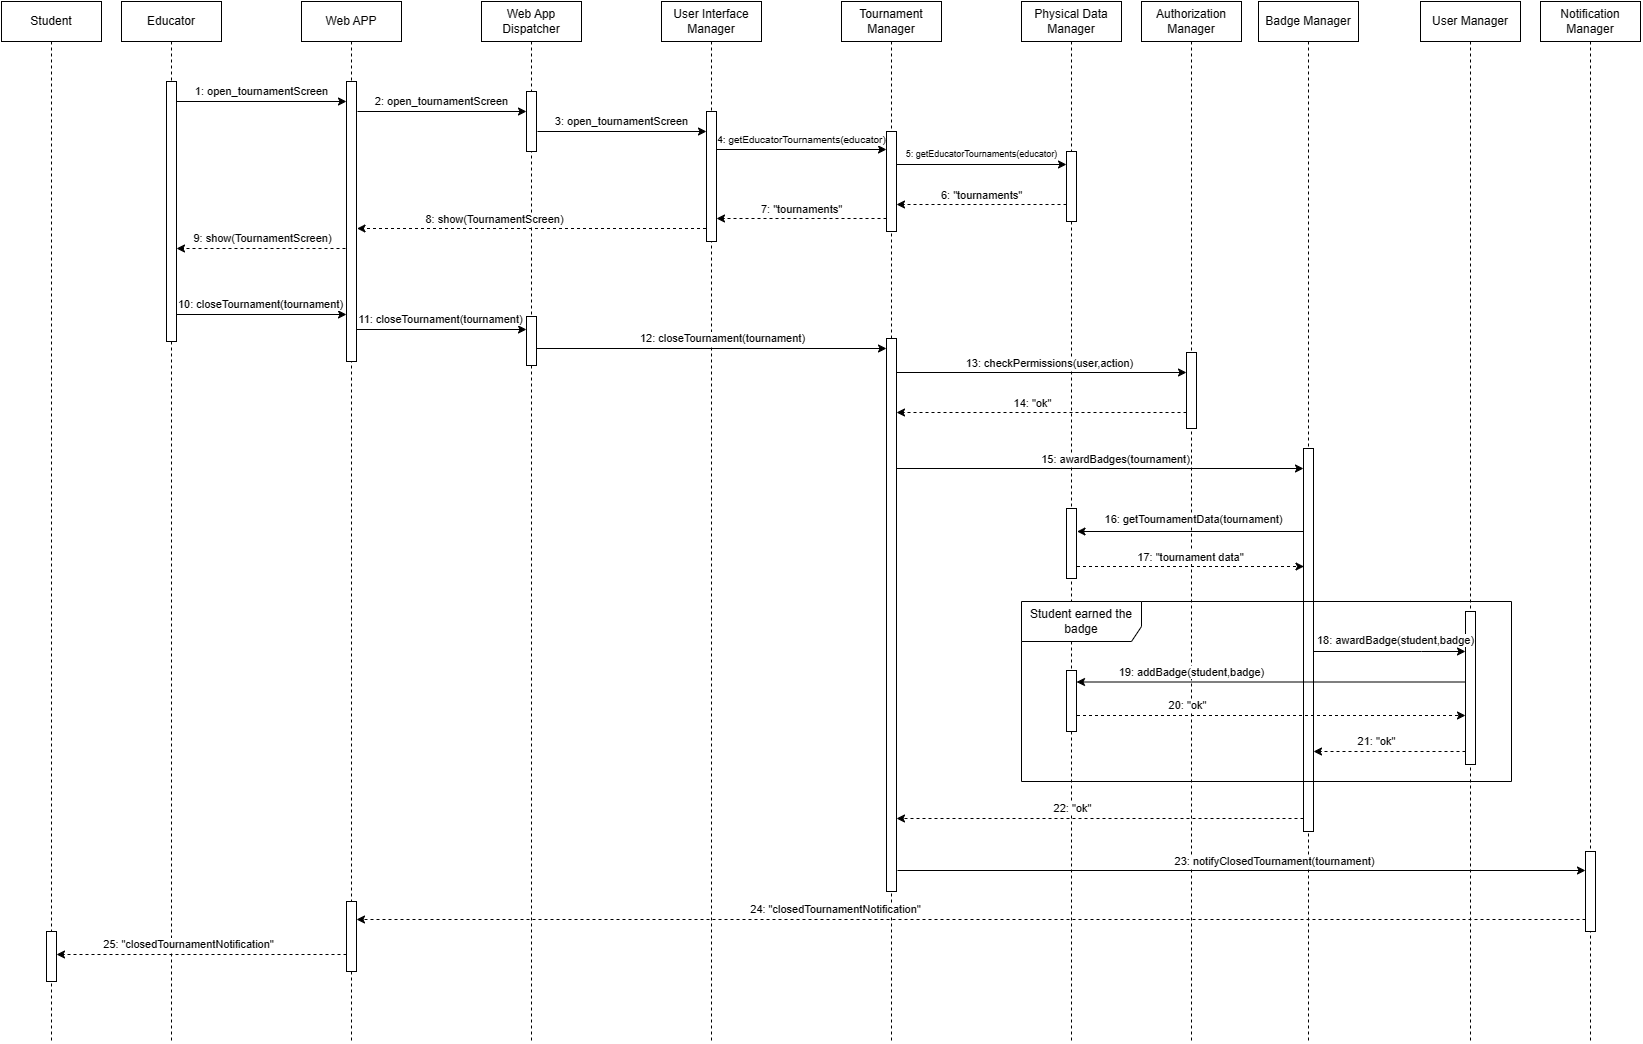
\includegraphics[width=1\linewidth]{Images/RV11.png}
        \caption{Tournament closure and Badge obtaining runtime view}
        \label{fig:rv11}
    \end{figure}

    This sequence diagram shows all the actions performed when an educator closes a tournament. After the educator selects the tournament to close from the "tournaments" page, the request is sent to the Tournament Manager that performs the required authorization checks. The Badge Manager is then responsible for collecting all the necessary data and checking, for each student subscribed to the tournament, if the constraints for winning each of the badges (defined during the tournament creation) are respected. If so, the badge is sent to the User Manager, which is responsible for adding the badge to the student's profile. At the end of the badge assignation process, the tournament is officially closed and a notification is sent to all the registered students.

    \newpage

    \item \textbf{Student Profile Visualization:}

    \begin{figure}[H]
        \centering
        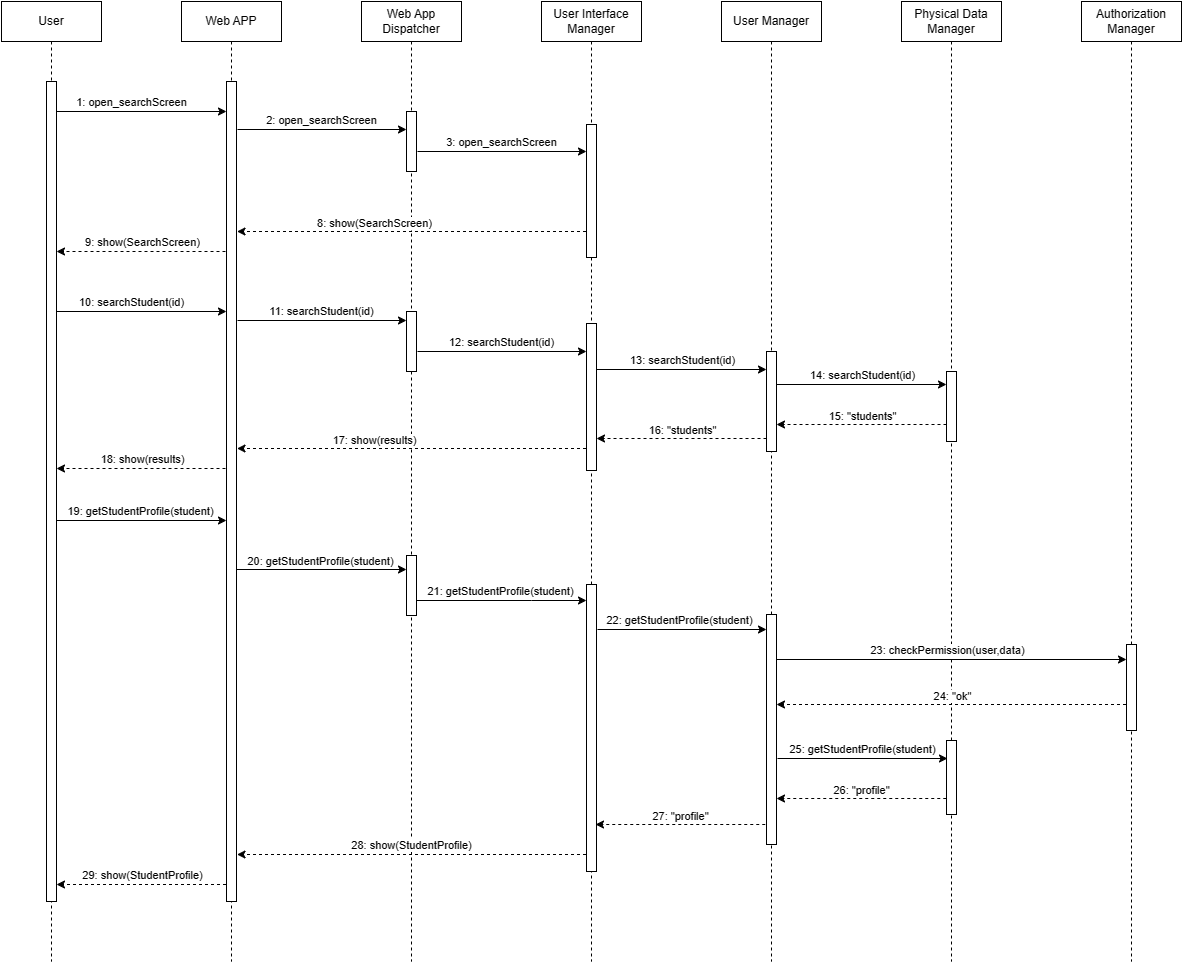
\includegraphics[width=1\linewidth]{Images/RV15.png}
        \caption{Student Profile Visualization runtime view}
        \label{fig:rv15}
    \end{figure}

    This sequence diagram shows all the actions performed when and user (either a student or an educator), requests the profile of a student, containing information such as the badges earned by the student. The user first enters the "search" page. From there, the user insert an identification of the requested student (i.e. the username or part of it). The request is sent to the User Manager, which in turn provides the set of students corresponding to the provided id. Once the list of students has been displayed to the user, they select the students whose profile they are interested in. The request is again forwarded to the User Manager, that after an authorization check returns to the User Interface Manager the student's data. Finally, the User Interface Manager prepares the content to be provided to the user.

\end{itemize}

\newpage

 \subsection{Component Interfaces}

 This section contains the functionalities provided by each interface to the other components. The lists include both generic methods offered in order to perform a wide set of operations, and case-specific methods employed for a clear and efficient usage of the provided functionalities.

 \begin{itemize}

    \item \textbf{Web App Dispatcher:}
    \begin{itemize}
     \item handleRequest(request)
    \end{itemize}
    
    \item \textbf{User Manager:}
    \begin{itemize}
     \item checkStudentExistence(email, username)
     \item checkEducatorExistence(email, username)
     \item createStudent(email, username, password, student\_data)
     \item createEducator(email, username, password, educator\_data)
     \item getStudentData(email)
     \item getEducatorData(email)
     \item updateStudentData(email, student\_data)
     \item updateEducatorData(email, educator\_data)
     \item awardBadge(student\_email, badge)
     \item deleteStudentData(email)
     \item deleteEducatorData(email)
    \end{itemize}

    \item \textbf{Registration Manager:}
    \begin{itemize}
     \item handleStudentRegistrationCredentials(email, username, password)
     \item handleEducatorRegistrationCredentials(email, username, password)
     \item checkRegistrationCredentialsCorrectness(email, username, password)
    \end{itemize}

    \item \textbf{Login Manager:}
    \begin{itemize}
     \item handleStudentLoginCredentials(username, password)
     \item handleEducatorLoginCredentials(username, password)
     \item checkLoginCredentialsCorrectness(username, password)
    \end{itemize}

    \item \textbf{Authorization Manager:}
    \begin{itemize}
        \item checkPermission(user, action)
        \item grantPermission(user, action)
        \item revokePermission(user, action)
    \end{itemize}

    \item \textbf{Tournament Manager:}
    \begin{itemize}
        \item getTournaments(search\_filters)
        \item getStudentTournaments(student)
        \item getEducatorTournaments(educator)
        \item createTournament(name, creator, badges, tournament\_data)
        \item inviteEducator(educator, tournament)
        \item createBattle(battle\_data)
        \item registerStudent(student, tournament)
        \item createTeam(students, battle)
        \item updateTournamentRank(battle, rank)
        \item closeTournament(tournament)
        \item getTournamentRank(tournament)
        \item getTournamentData(tournament)
        \item updateTournamentData(tournament)
        \item deleteTournamentData(tournament)
    \end{itemize}

    \item \textbf{Battle Manager:}
    \begin{itemize}
        \item getBattles(search\_filters)
        \item getStudentBattles(student)
        \item getEducatorBattles(educator)
        \item createBattle(name, creator, description, parameters, software\_components, battle\_data)
        \item addPendingTeam(students, battle)
        \item acceptInvitation(student, team, battle)
        \item checkTeam(team)
        \item handleNewSubmission(submission, battle)
        \item calculateBattleRank(evaluations, battle)
        \item getBattleLastSubmissions(battle)
        \item handleEducatorEvaluations(evaluations, battle)
        \item getBattleRank(battle)
        \item getBattleData(battle)
        \item updateBattleData(battle)
        \item deleteBattleData(battle)
    \end{itemize}

\newpage
    \item \textbf{GitHub Integration Manager:}
    \begin{itemize}
        \item createRepository(battle)
        \item setupWorkflow(repository, students)
        \item closeRepository(repository)
    \end{itemize}


    \item \textbf{Automated Evaluation Manager:}
    \begin{itemize}
        \item evaluateSubmission(code, software\_components, eval\_parameters)
    \end{itemize}

    \item \textbf{User Interface Manager:}
    \begin{itemize}
        \item preparePageContent(page, content)
        \item loginPage()
        \item registerAsStudentPage()
        \item registerAsEducatorPage()
        \item loginAsStudentPage()
        \item loginAsEducatorPage()
        \item studentHomePage(student\_data)
        \item educatorHomePage(educator\_data)
        
        \item studentTournamentsPage(student, tournaments)
        \item educatorTournamentsPage(educator, tournaments)

        \item studentBattlesPage(student, battles)
        \item educatorBattlesPage(educator, battles)

        \item inviteEducatorPage(educator, tournament)
        \item tournamentBadgesPage(educator, tournament)
        \item battleFinalSubmissionsPage(educator, battle\_final\_submissions)
        \item battleRankPage(battle\_info)
        \item searchPage()
        \item tournamentRankPage(tournament\_info)
        \item studentProfilePage(student\_info)
        
    \end{itemize}

    \item \textbf{Badge Manager:}
    \begin{itemize}
        \item awardBadges(tournament)
        \item checkBadge(student, badge, tournament)
    \end{itemize}

    \newpage

    \item \textbf{Notification Manager:}
    \begin{itemize}
        \item sendNotification(email, content)
        \item sendConfirmationLinkEmail(email)
        \item sendConfirmationEmail(email)
        \item notifyNewTournament(tournament)
        \item notifyInvitation(team, emails)
        \item notifyNewBattle(battle)
        \item notifyBattleClosure(battle)
        \item notifyTournamentClosure(battle)
    \end{itemize}

    \item \textbf{Physical Data Manager:}
    \begin{itemize}
        \item executeQuery(query)
        \item insert(data)
        \item select(query)
        \item update(data)
        \item delete(data)
    
        \item createStudent(email, username, password, student\_data)
        \item getStudentData(student)
        \item updateStudentData(student, student\_data)
        \item addBadge(student, badge)
        \item deletStudentData(student)

        \item createEducator(email, username, password, educator\_data)
        \item getEducatorData(educator)
        \item updateEducatorData(educator, educator\_data)
        \item deletEducatorData(educator)

        \item createTournament(name, creator, badges, tournament\_data)
        \item getTournaments(search\_filters)
        \item getStudentTournaments(student)
        \item getEducatorTournaments(educator)
        \item getTournamentRank(tournament)
        \item updateTournamentRank(battle, rank)
        \item getTournamentData(tournament)
        \item updateTournamentData(tournament)
        \item deleteTournamentData(tournament)

        \item createBattle(name, creator, description, parameters, software\_components, battle\_data)
        \item getBattles(search\_filters)
        \item getStudentBattles(student)
        \item getEducatorBattles(educator)
        \item getFinalSubmissions(battle)
        \item storeSubmission(submission, battle)
        \item getBattleRank(battle)
        \item updateBattleRank(battle, rank)
        \item getBattleData(battle)
        \item updateBattleData(battle)
        \item deleteBattleData(battle)
        
    \end{itemize}
    
 \end{itemize}

 \subsection{Selected Architectural Styles and Patterns}
 This chapter talks about the architectural design choices that define the CodeKataBattle platform, highlighting patterns that contribute to its robustness and flexibility.
 
\begin{itemize}
    \item \textbf{3-Tier Architecture:} \\
    The CKB platform is based on a 3-tier architecture, that organize its system’s components logically and physically into three distinct tiers: presentation, application, and data tier. Thanks to the modularization, this architecture allows for a clear division of responsibilities, promotes modularity and scalability, facilitating efficient development and maintenance, and guarantees a higher flexibility by allowing to develop and update a specific part of the system at time. 
    
    \item \textbf{Chain of Responsibility Pattern:} \\
    It's employed to establish a chain of handler objects. Each handler has the capability to process a request or pass it along the chain. This pattern enhances flexibility by allowing multiple objects to handle a request without the sender needing to specify the exact handler. It’s particularly useful for processing various user requests and system events, enabling a modular and scalable approach to request handling. In CKB system the first chain link is the dispatcher, which is in charge of passing the request to one or more components. Each component then handles the request, forwarding it to the other components if necessary.

    \item \textbf{Microservices Architecture:} \\
    The CKB platform's architecture is based on a microservices architectural style. Microservices break down the system into independently deployable and scalable services, enhancing agility and adaptability. Each component of the system embodies a small set of functionalities related to single entities (tournaments, battles, ...), and the common operations performed by each component, such as data retrieval or the preparation of the user interface to display, are allocated to specialized components.

    \item \textbf{Strategy Pattern for Badges:} \\
    For badge management, the CKB platform incorporates the strategy design pattern. It defines a family of algorithms, encapsulates each algorithm, and makes them interchangeable. In the context of badges, it allows educators to define scoring algorithms dynamically, that can be changed at run-time, influencing how badges are awarded. The Badge Manager component is then responsible for employing the defined checks in order to award badges to student, based on the large set of rules offered to the educators.

    \item \textbf{Observer Pattern for Subscriptions:} \\
    For subscription management, the CKB platform uses the observer pattern. This pattern establishes a one-to-many dependency between objects, ensuring that when one object changes state, all its dependents are notified and updated automatically. Applied to subscriptions, this enables real-time notifications to students about upcoming battles and changes in tournament status.

    \item \textbf{Command-Query Separation (CQS):} \\
    This pattern separates the methods that modify data (commands) from the methods that return data (queries) to improve clarity and maintainability. Commands and queries are distinct, preventing unintended side effects when retrieving information. It is employed in the Physical Data Manager: the component offers, in addition to interfaces for generic queries, specific types of requests and commands for each case. 
    
    \item \textbf{State Pattern:} \\
    It is applied to enable an object to change its behavior when its internal state changes. This pattern is particularly useful when an object has different behaviors in response to various states. In CKB, it’s employed to manage the lifecycle of battles and tournaments, allowing them to transition between states and modify the response to certain requests based on them. 

    \item \textbf{Façade Pattern:} \\
    The façade pattern is applied to simplify the interactions between complex subsystems offering a unified interface. Within the CKB system, it’s used in the implementation of the dispatcher component. It encapsulates the underlying complexities of the system to hide the complexity of the application server to the client application, that has a user-friendly interface, and reducing dependencies. In fact, this also provides a simple interface for users.

    \item \textbf{Mediator Pattern:} \\
    The mediator pattern manages the communication between all the different components without direct dependencies, to facilitate communication and coordination between them. In the CKB platform, it reduces coupling, promotes flexibility and easiness of modification, allowing changes in one component to have minimal impact on others. It is interposed between two or more objects and encapsulates their communication, so that they cannot know each other’s implementation details. In addition, it not only enhances flexibility but also simplifies the addition of new features and functionalities.

\end{itemize}

\subsection{Other Design Decisions}
\begin{itemize}
    \item \textbf{Load Balancer and Server Replicas:} \\
    To strengthen system availability, the CKB platform integrates three load balancers that distribute incoming traffic across multiple server replicas. This setup not only optimizes resource utilization but also mitigates the risk of downtime due to server failures. The load balancer intelligently redirects requests, ensuring a balanced and efficient distribution of workloads among server instances. In case of a server failure, the load balancer redirects traffic to healthy replicas, minimizing interruptions and providing users with continuous access to the platform.
    \item \textbf{Distributed Database on a Cluster:} \\
    At the database level, the CKB platform adopts a unique logical database distributed on a cluster of physical databases. This architecture involves the distribution of database instances across multiple nodes, forming a resilient cluster. In the event of a database node failure, the distributed nature of the cluster ensures that other nodes take over, preventing service interruptions. This approach not only improves fault tolerance but also supports scalability and performance optimization.
\end{itemize}
The combination of load balancing for system components and a distributed database cluster strengthens the CKB platform's availability. By distributing workloads and data across multiple nodes, the platform remains robust to potential malfunctioning, offering users uninterrupted access and reliable performance. 

